\section{Project 2 - Spatial Enhancement Methods}
\subsection{Project Proposal}
Implement the image spatial enhancement task showed in text book Figure 3.43. The steps involve Laplacian
filter, Sobel filter, average filter and power law transformation.

\subsection{Preliminaries}
\subsubsection{Basic Spatial Filtering}
In general, linear spatial filtering of an image of size $M\times N$ with a filter of size $m \times n$ is \begin{equation} g(x,y)=\sum_{s=-a}^a \sum_{t=-b}^b  w(s,t)f(x+s,y+t) \end{equation} where $a=(m-1)/2$ and $b=(n-1)/2$. There are two closely related concepts related to spatial filtering.
One is \emph{correlation} and the other is \emph{convolution}. Correlation of filter $w(x, y)$ is defined as \begin{equation}\sum_{s=-a}^a \sum_{t=-b}^b  w(s,t)f(x+s,y+t) \end{equation} while convolution is defined as \begin{equation} \sum_{s=-a}^a \sum_{t=-b}^b  w(s,t)f(x-s,y-t) \label{eq:convdefine}\end{equation}
 The confusion point is that we usually call spatial filter as convolution filter, convolution mask or convolution kernel but the terms are not necessarily refer to the true convolution operation defined in Eq.\ref{eq:convdefine}. 

\subsubsection*{Smoothing spatial filters}
Smoothing filters are used for blurring and for noise reduction. The simplest smoothing filter is averaging filters, which is also called lowpass filter. $M \times N$ averaging filter can be represented as \begin{equation} g(x,y)=\frac{\sum_{s=-a}^a \sum_{t=-b}^b w(s,t)f(x+s,y+t)}{\sum_{s=-a}^a \sum_{t=-b}^b w(s,t)} \end{equation} The simple idea of filter size choosing is that choose the approximately the same size of the noisy you want to reduce. Average filter is an example of linear spatial filters. There are also nonlinear order-static spatial filters using the ranking information of each pixel. We will talk about order-static filters in \emph{Project 8}. 

\subsubsection*{Sharpening spatial filters}
The principal objective of sharpening is to highlight transitions in intensity. Because averaging is analogous to integration, it is logical to conclude that sharpening can be accomplished by spatial differentiation. Thus we consider the sharpening filters based on first- and second-order derivatives. \newline
\textbf{Second-order derivatives - the Laplacian} \newline
Laplacian is defined as \begin{equation} \nabla^2 f=\frac{\partial^2f}{\partial x^2}+\frac{\partial^2f}{\partial y^2} \end{equation} In x-direction and y-direction we have \begin{equation} \frac{\partial^2f}{\partial x^2} = f(x+1,y)-f(x,y)-(f(x,y)-f(x-1,y))=f(x+1,y)+f(x-1,y)-2f(x,y) \end{equation} \begin{equation} \frac{\partial^2f}{\partial y^2} = f(x,y+1)-f(x,y)-(f(x,y)-f(x,y-1))=f(x,y+1)+f(x,y-1)-2f(x,y) \end{equation}
Thus we get the discrete Laplacian of two variables:
\begin{equation}
nabla^2 f(x,y)=f(x+1,y)+f(x-1,y)f(x,y+1)+f(x,y-1)-4(x,y)
\label{eq:lapfilter}\end{equation} Based on Eq.\ref{eq:lapfilter} we have 4 masks displayed in Fig.\ref{fig:lapfilter}. The basic way we use Laplacian for image sharpening is \begin{equation} g(x,y)=f(x,y)+c\left[ \nabla^2 f(x,y) \right] \end{equation} where $c=1$ if we use Fig.\ref{fig:lap3} or Fig.\ref{fig:lap4}. 

\begin{figure}[h!]
	\centering
	\begin{subfigure}[b]{0.2\linewidth}
		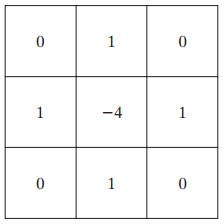
\includegraphics[width=\linewidth]{myfigure/p2/lap-1.png}
		\caption{}
		\label{fig:lap1}
	\end{subfigure}
	\begin{subfigure}[b]{0.2\linewidth}
    	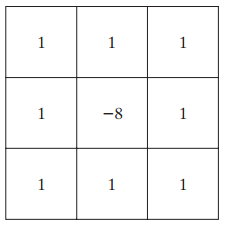
\includegraphics[width=\linewidth]{myfigure/p2/lap-2.png}
		\caption{}
		\label{fig:lap2}
  	\end{subfigure}
  	\begin{subfigure}[b]{0.2\linewidth}
		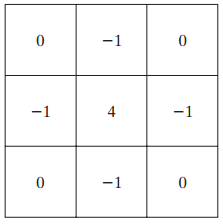
\includegraphics[width=\linewidth]{myfigure/p2/lap-3.png}
		\caption{}
		\label{fig:lap3}
	\end{subfigure}
	\begin{subfigure}[b]{0.2\linewidth}
    	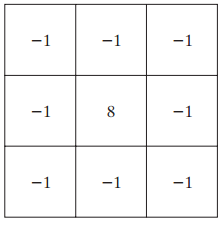
\includegraphics[width=\linewidth]{myfigure/p2/lap-4.png}
		\caption{}
		\label{fig:lap4}
  	\end{subfigure}
  	\caption{4 Laplacian masks. \textbf{(a)}Direct implementation of Eq.\ref{eq:lapfilter}. \textbf{(b)}Extent (a) by adding two diagonal terms. \textbf{(c)(d)} sign inverse of (a)(b) relatively. More common in practice.}
  	\label{fig:lapfilter}
\end{figure}

\textbf{First-order derivatives - the gradient} \newline
First-order derivatives in image processing using the magnitude of the gradient. The gradient vector is \begin{equation} \nabla f \equiv \text{grad}(f) \equiv \left[ \begin{array}{c} g_x \\ g_y \end{array}\right] = \left[ \begin{array}{c} \frac{\partial f}{\partial x} \\ \frac{\partial f}{\partial y} \end{array} \right] 
\end{equation}
The magnitude of vector $\nabla f$ defined as \begin{equation}M(x,y)=mag(\nabla f) =  \sqrt{g_x^2 + g_y^2} \approx |g_x| + |g_y| \end{equation} is the value of the rate of change in the direction of the gradient vector. The second = is a frequently used approximate to avoid square roots. A widely used approximate filter masks implementing gradient is Sobel defined as \begin{equation} g_x = \frac{\partial f}{\partial x} =  (z_7+2z_8+z_9) - (z_1+2z_2+z_3)\end{equation} and \begin{equation} g_y = \frac{\partial f}{\partial y} =  (z_3+2z_6+z_9) - (z_1+4z_2+z_7)\end{equation}
$3\times 3$ Sobel filter is displayed in Fig.\ref{fig:sobel}
\begin{figure}[h!]
	\centering
	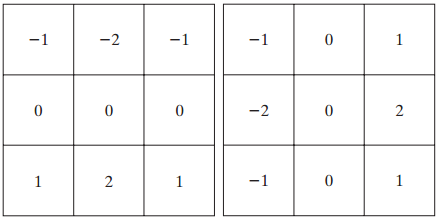
\includegraphics[scale=0.6]{myfigure/p2/sobel.png}
	\caption{$3\times 3$ SObel mask. Left is on x direction, right is on y direction.}
	\label{fig:sobel}
\end{figure}

\subsection{Experiment - Combining Spatial Enhancement}
We conduct the experiment on the Fig.2.3a image of whole body bone scan. Our goal is to enhance this image by sharpening it and by bringing out more of the skeletal detail. The narrow dynamic ranging of the intensity levels and high noise content make this problem difficult. The process and result images are displayed in Fig.\ref{fig:abcd} and Fig.\ref{fig:efgh}. Here, I describe the detail process of the enhancement. \newline
We first use Laplacian with the mask in Fig.\ref{fig:lap4} to extract the sharp transitions in intensity. Note that Fig.2.3b is a scaled result because the numerical matrix result contains negative values which can not be visualized as image by matlab default function. After obtaining Laplacian, we add Laplacian(not the scaled one by the real laplacian) to the original image to get the sharpened Fig.2.3c. This step is just follow Eq.\ref{eq:lapfilter}. In Fig.2.3d we compute the Sobel gradient of original image using masks in Fig.\ref{fig:sobel}. Edges are more dominant than ones in Laplacian. In Fig.2.4e we use $5 \times 5 $averaging filter to smooth the Sobel gradient for noisy reduction purpose. It’s not proper to use median filter because medical image processing requires high level of convince. In Fig.2.4f, we multiply the Laplacian with Sobel. Multiply seems like a strange operation but we can consider it as use Sobel to mask Laplacian in order to strengthen edges and reduce noisy. In Fig.2.4g we sum up the product and the original image. Finally in Fig.2.4h we increase the dynamic range of the sharpened image by powerlaw transformation which is defined as
\begin{equation} s-cr^\gamma \end{equation} where we use $\gamma=0.5$ and $c=1$. We use $\gamma <1$ to spread the intensity level and note that histogram equalization would not give use satisfying result as discussed in Project 1.

\subsection{Discussion}
We finally get a satisfy result in the Fig.2.4h which shows significant new visible features. There are two tricks we should pay attention to. First, the operations may produce intensity levels out of the range $[0,255]$. In this kind of cases, a direct matlab command \emph{imshow()} will cause problem. So we have to use scale function. While coding, I made a mistake that I didn’t take the numerical type into consideration. I gain an experience that before computation, transform the matrix type to double at first.

\subsection{Implementation}
Here I paste the key parts of my matlab implementation.
\lstset{language=Matlab}
\begin{lstlisting}
function [ imgg ] = replicate_padding( imgf, pad )
%REPLIACTE_PADDING
% imgf - img to be padded, pad - amount of padding 
[M, N] = size(imgf);
% repmat(mat, row_rep, col_rep);
top = repmat(imgf(1, :), pad, 1);
button = repmat(imgf(M, :), pad, 1);
left = repmat(imgf(:, 1), 1, pad);
right = repmat(imgf(:, N), 1, pad);
lt = repmat(imgf(1,1), pad, pad);
rt = repmat(imgf(1,N), pad, pad);
lb = repmat(imgf(M,1), pad, pad);
rb = repmat(imgf(M,N), pad, pad);
imgg = [lt, top, rt; left, imgf, right; lb, button, rb];
end
\end{lstlisting}

\lstset{language=Matlab}
\begin{lstlisting}
function [ scale_imgg, imgg] = b_laplacian_scale( imgf )
%B_LAPLACIAN_SCALE 
[M, N] = size(imgf);
% padding
f = replicate_padding(imgf, 2);
f = double(f);
% laplacian
mask = [-1 -1 -1; -1 8 -1; -1 -1 -1];
g = zeros(M+4, N+4);
for x = (2 : M+3)
    for y = (2 : N+3)
        g(x, y) = sum(sum(f(x-1:x+1, y-1:y+1) .* mask));
    end
end
imgg = g(3:M+2, 3:N+2); % laplacian result without scale
% scale
scale_imgg = scale255(imgg);
end
\end{lstlisting}
\lstset{language=Matlab}
\begin{lstlisting}
function [ imgg ] = d_sobel( imgf )
%D_SOBEL 
[M, N] = size(imgf);
f = replicate_padding(imgf, 2);
f = double(f); % double f
% Sobel
maskx = [-1 -2 -1; 0 0 0; 1 2 1];
masky = [-1 0 1; -2 0 2; -1 0 1];
gx = zeros(M+4, N+4);
gy = zeros(M+4, N+4);
for x = (2 : M+3)
    for y = (2 : N+3)
        gx(x, y) = sum(sum(f(x-1:x+1, y-1:y+1) .* maskx));
        gy(x, y) = sum(sum(f(x-1:x+1, y-1:y+1) .* masky));
    end
end
% new image: using abs
gx = abs(gx(3:M+2, 3:N+2));
gy = abs(gy(3:M+2, 3:N+2));
imgg = scale255(gx+gy);
end
\end{lstlisting}
\lstset{language=Matlab}
\begin{lstlisting}
function [ imgg ] = scale255( imgf )
%SCALE255 
% return is uint8 type
%imgf = double(imgf);
[M, N] = size(imgf);
K = 255;

minf = zeros(M, N) + min(min(imgf));
maxf = zeros(M, N) + max(max(imgf));
imgg = K * (imgf-minf) ./ (maxf - minf);
imgg = uint8(imgg);
end
\end{lstlisting}

\lstset{language=Matlab}
\begin{lstlisting}
function [ imgg ] = e_5x5_average( imgf )
%E_5X5_AVERAGE
[M, N] = size(imgf);
% padding
f = replicate_padding(imgf, 4);
f = double(f);
% 5x5 average
g = zeros(M+8, N+8);
for x = (3 : M+6)
    for y = (3 : N+6)
        g(x, y) = sum(sum(f(x-2:x+2, y-2:y+2))) / 25;
    end
end
imgg = g(5:M+4, 5:N+4); % laplacian result without scale
imgg = uint8(imgg);
end
\end{lstlisting}

\clearpage

\begin{figure}[h!]
	\centering
	\begin{subfigure}[b]{0.4\linewidth}
		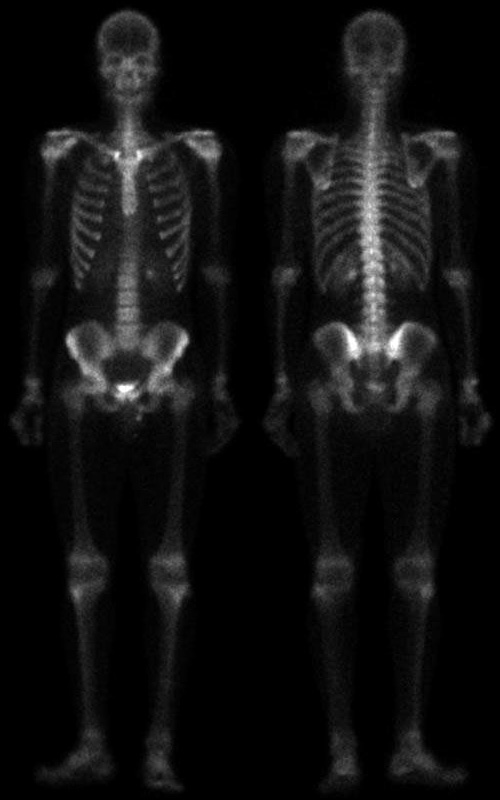
\includegraphics[width=\linewidth]{myfigure/p2/2-a.png}
		\caption*{(a)}
		\label{fig:2a}
	\end{subfigure}
	\begin{subfigure}[b]{0.4\linewidth}
    	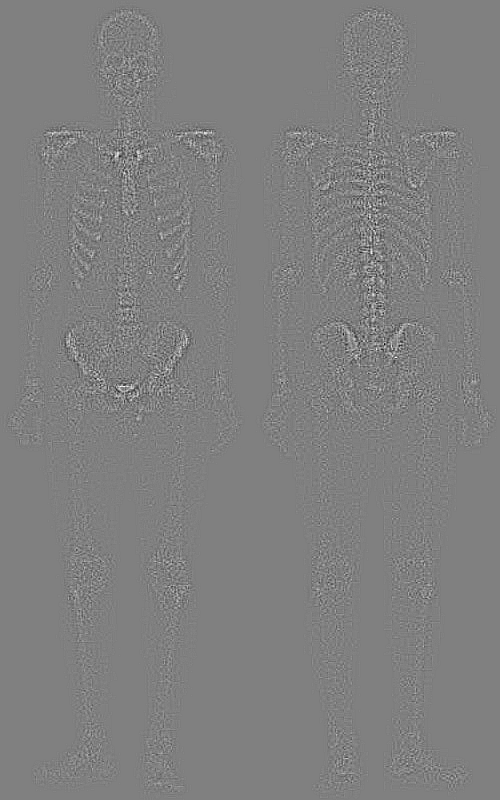
\includegraphics[width=\linewidth]{myfigure/p2/2-b.png}
		\caption*{(b)}
		\label{fig:2b}
  	\end{subfigure}
  	\begin{subfigure}[b]{0.4\linewidth}
		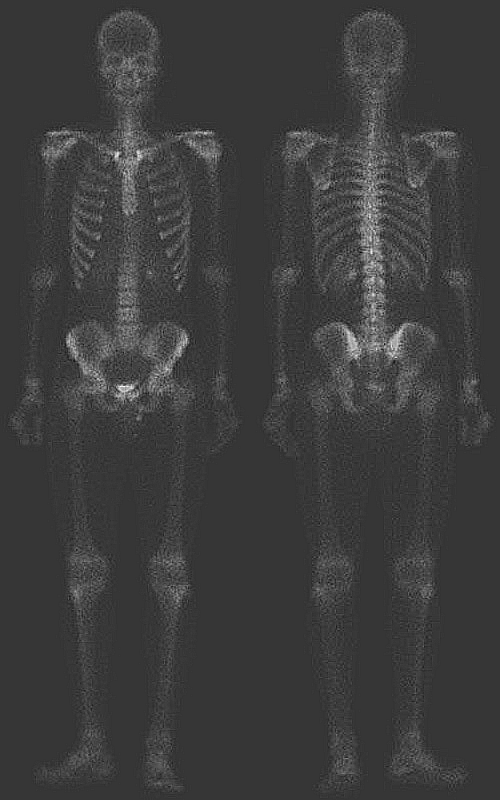
\includegraphics[width=\linewidth]{myfigure/p2/2-c.png}
		\caption*{(c)}
		\label{fig:2c}
	\end{subfigure}
	\begin{subfigure}[b]{0.4\linewidth}
    	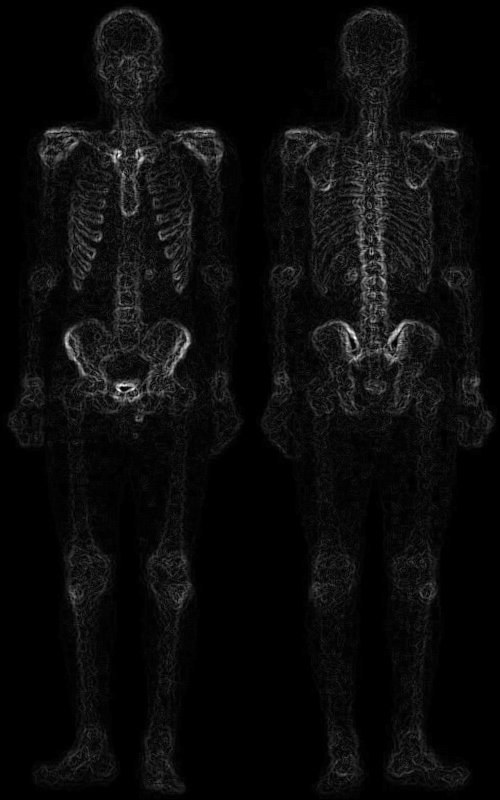
\includegraphics[width=\linewidth]{myfigure/p2/2-d.png}
		\caption*{(d)}
		\label{fig:2d}
  	\end{subfigure}
  	\caption{\textbf{a}Original image of whole body bone scan. \textbf{(b)}Laplacian of (a)(Rescaled to [0,255]). \textbf{(c)}Sharpened image obtained by add (a) and (c). \textbf{(d)}Sobel gradient of (a).}
  	\label{fig:abcd}
\end{figure}
\clearpage
\begin{figure}[h!]
	\centering
	\begin{subfigure}[b]{0.4\linewidth}
		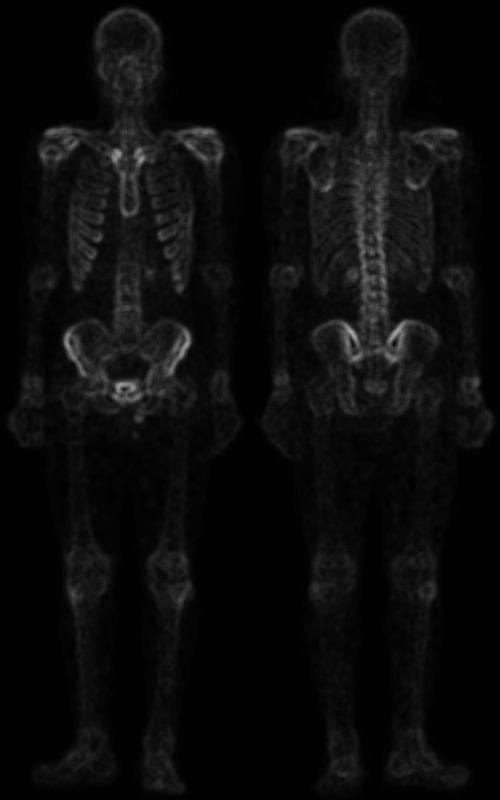
\includegraphics[width=\linewidth]{myfigure/p2/2-e.png}
		\caption*{(e)}
		\label{fig:2e}
	\end{subfigure}
	\begin{subfigure}[b]{0.4\linewidth}
    	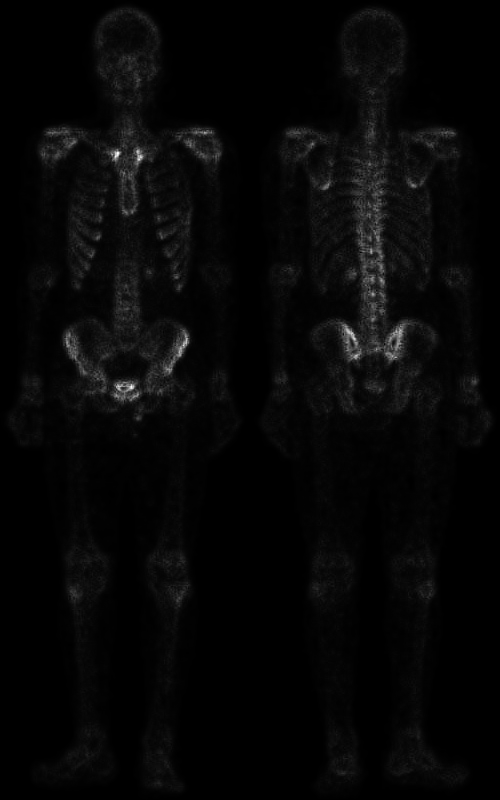
\includegraphics[width=\linewidth]{myfigure/p2/2-f.png}
		\caption*{(f)}
		\label{fig:2f}
  	\end{subfigure}
  	\begin{subfigure}[b]{0.4\linewidth}
		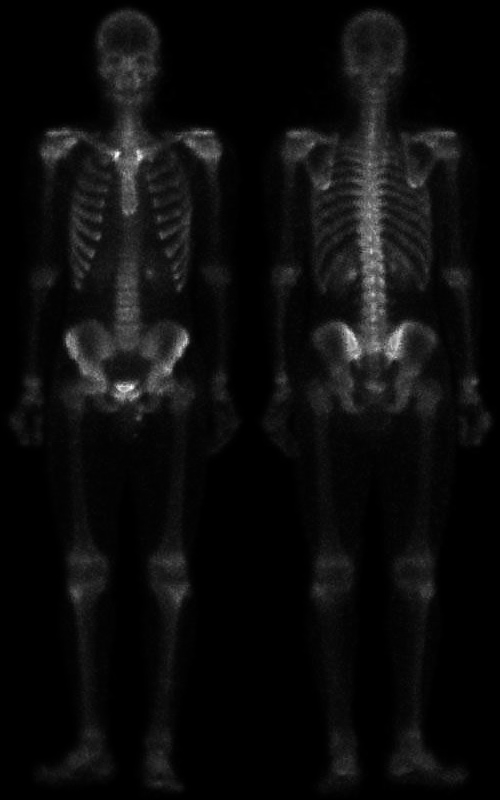
\includegraphics[width=\linewidth]{myfigure/p2/2-g.png}
		\caption*{(g)}
		\label{fig:2g}
	\end{subfigure}
	\begin{subfigure}[b]{0.4\linewidth}
    	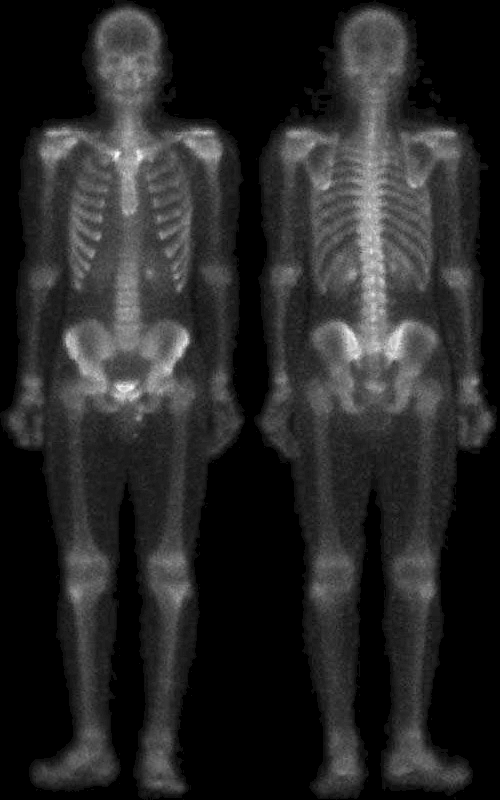
\includegraphics[width=\linewidth]{myfigure/p2/2-h.png}
		\caption*{(h)}
		\label{fig:2h}
  	\end{subfigure}
  	\caption{\textbf{(e)}Sobel image smoothed with $5\times 5$ averaging filter. \textbf{(f)}Mask image formed by the product of (c) and (e). \textbf{(g)}Sharpened image obtained by applying a power-law transformation to (g). \textbf{(h)}Compare (g) and (h).}
  	\label{fig:efgh}
\end{figure}


